\chapter{Simulation: localisation and transport}

We will now employ the theoretical framework constructed above, and numerically study the transport properties of complex networks using the response and transmission matrix formalism. The simulations are done in MATLAB, and are built upon a library written by Michele Gaio \cite{Gaio2017}. 

\section{Setup}
In our simulations we look at two types of random network geometries: Delaunay graphs and Voronoi graphs. Both types are generated by seeding a 2D plane with uniform-random distributed points; these are then used either as the vertices in a Delaunay triangulation of the plane, or cell centres in a Voronoi diagram. Given the same set of seed points, the resulting Delaunay and Voronoi graphs are dual to each other, i.e. each node in one graph corresponds to a face (a region enclosed by edges) in the other. Note that given $N$ seed points, the resulting Delaunay graph will have $N$ nodes, while the Voronoi graph will have $\alpha N$ nodes, with typical $1.5<\alpha<2$.


We work with rectangular-shaped networks, with open (external) edges on the left and right end. Since experimentally one would not be able to use the same open edge for both input and output, we select the open edges on the left of a network as inputs, and those on the right as outputs. This means the resulting transmission matrices are sub-unitary. 

The networks are normalised to have height $1$ and varying widths, which we refer to as the \textit{depth} ($D$). Actual physical size of the networks are set by putting conversion factors into the wavenumber $k$. For example, if we want to model $700nm$ light on a $200\mu m \times 200 \mu m$ network, $k=2\pi n/\lambda = 4\pi/(0.7/200) \approx 3590$, where we have set $n=2$. Fig.\ref{fig:example_delaunay} and Fig.\ref{fig:example_voronoi} show examples of random networks.
\begin{figure}[h]
  \centering
    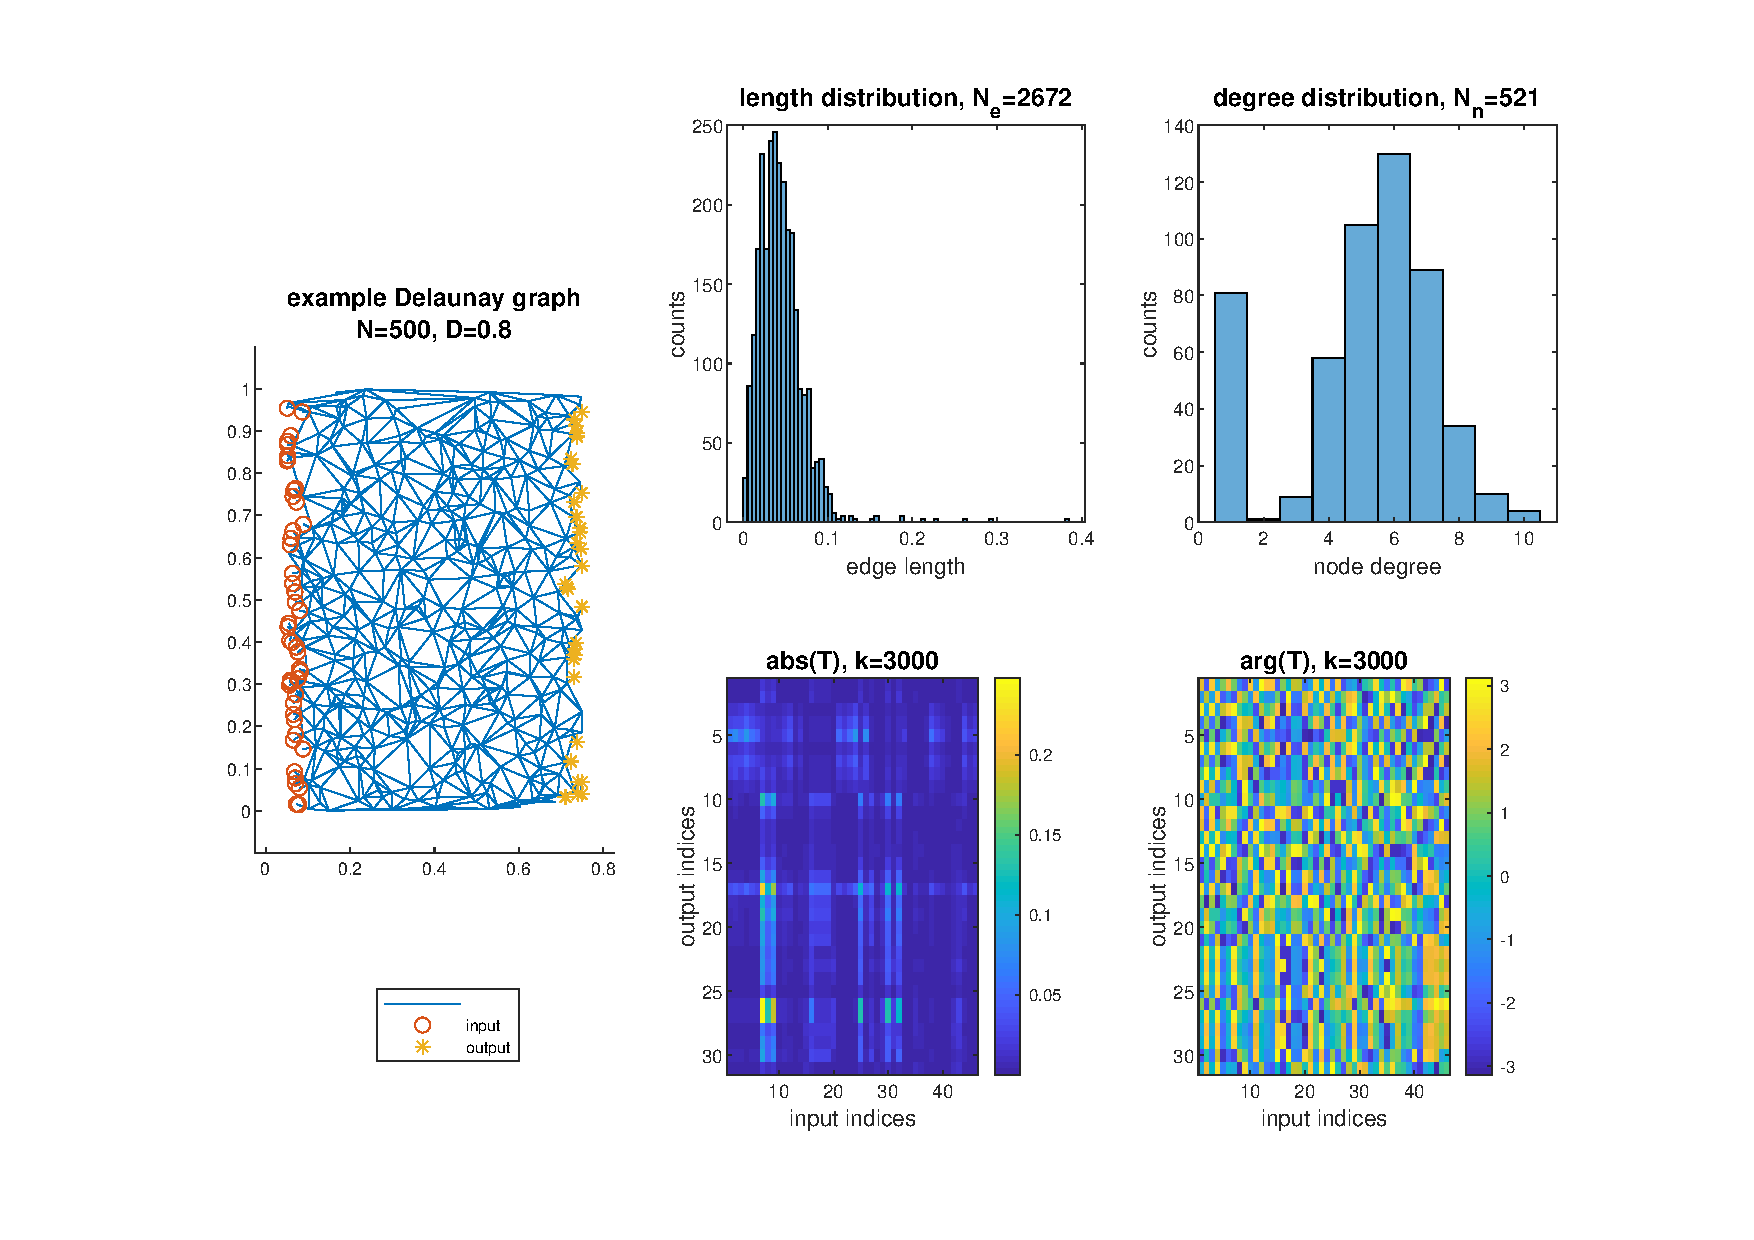
\includegraphics[width=\textwidth]{ch3/fig3/example_d.pdf}
    \caption{An example Delaunay graph. As a reminder, $N$ is the number of seed points, $D$ is the depth (width) of the graph, $N_e$ is the number of edges, $N_n$ is the number of nodes. Here $N_n \neq N$ because we have opened the graph on the left and right sides and added external nodes. The two plots in the bottom-right show the transmission matrix $T$ for $k=3000$: we see that $abs(T)$ which corresponds to transmitted intensity is sparse, while the output phase $arg(T)$ is fully randomised across $[-\pi,\pi]$.} 
    \label{fig:example_delaunay}
\end{figure}

\begin{figure}[h]
  \centering
    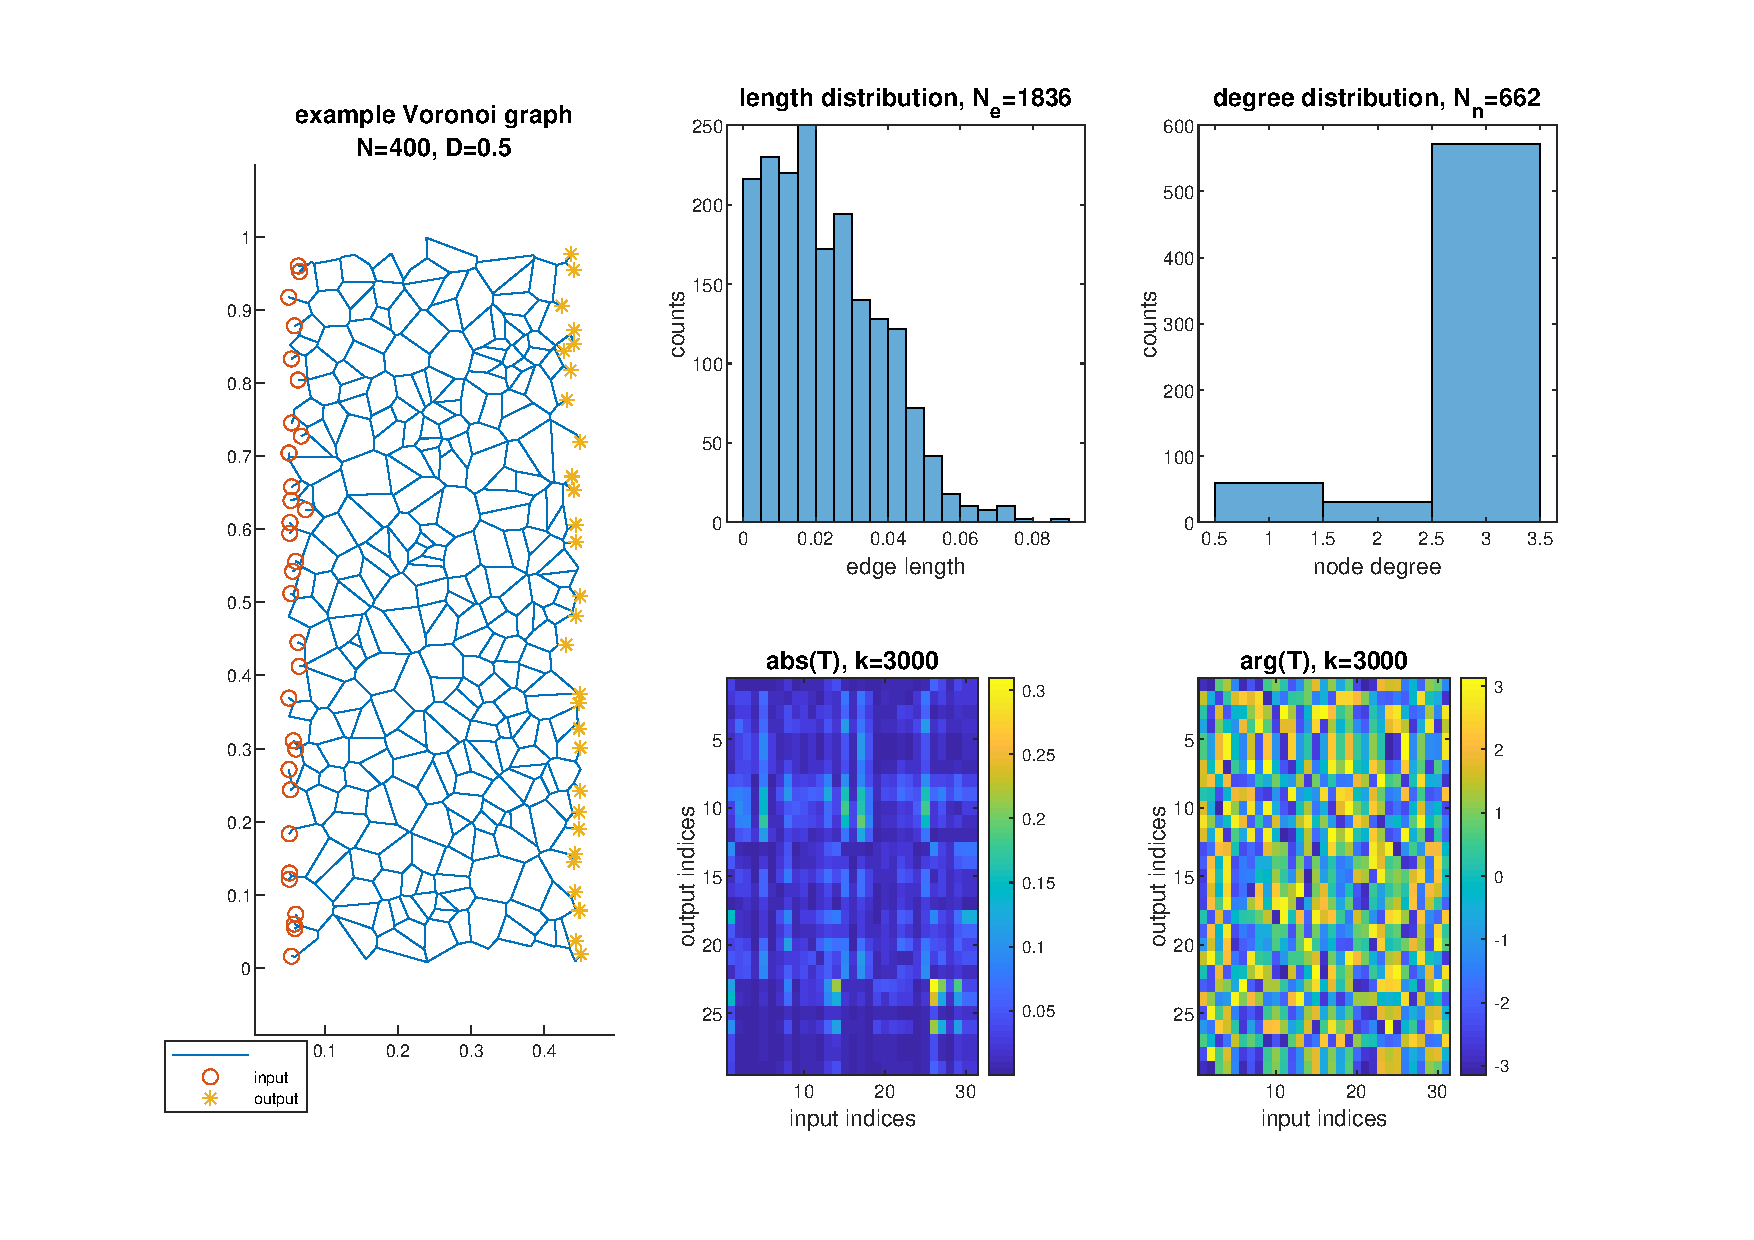
\includegraphics[width=\textwidth]{ch3/fig3/example_v.pdf}
    \caption{Same analysis as above, but for a Voronoi graph of different size. Here the discrepancy between $N_n$ and $N$ is larger due to the way in which Voronoi graphs are generated.} 
    \label{fig:example_voronoi}
\end{figure}

The randomness of the graphs (and the scattering process) is thus captured in the distribution of network edge lengths and node degrees. Roughly, the nodes randomise the intensity of back-scattering, while the edges randomise the relative phases between back-scattered waves. 
In the following sections, we will start by analysing the transport behaviour of classical electromagnetic waves, then adapt the simulation to quantum light.

\section{Scaling theory and localisation}
In the previous chapter we have constructed a bottom-up picture of the complex networks. To study multiple scattering and localisation properties, we need to take a top-down, statistical approach. There are several ways to characterise the localisation regime of a disordered system; the one we will focus on is scaling theory. The background on scaling theory in this section is based largely on \cite{Muller2011}. %\cite{Muller2011,Abrahams1979}.

A short note on dimensionality is necessary before we proceed. Up until this point the networks have been described as 2D systems since they are planar graphs embeded in 2D space. However, they are not necessarily equivalent to 2D disordered systems in the context of multiple scattering. Within nanophotonic systems, multiple-scattering can be modelled with a network geometry under the coupled-dipole approximation \cite{Yurkin2007}. On the other hand, multiple scattering is usually achieved by sending a plane wave into a bulk material, with disorder along one \cite{Sheinfux2017}, two \cite{Schwartz2007} or three \cite{Wiersma1997} dimensions. This is different from our setup where plane waves are injected independently into each input edge. Thus the complex network can be seen as either a discretised model for 2D disordered media with wavefront shaping abilities, or a quasi-1D system where the different spatial channels are coupled via network modes. It is for this reason we only vary the network depth $D$ in one dimension when simulating scaling properties of the system.

A scaling theory characterises the a physical system's properties as a function of its size $L$. In our example, $L \sim D$. Scaling theory studies \textit{universal} properties, i.e. properties that hold statistically across many realisations of the same random system, characterised by its level of disorder. Strong localisation is manifested by the scaling of transmission intensity, which we denote $I_t$:
\begin{equation}
    \label{eq:scaling}
    I_t(L) = e^{-L/\xi_{loc}}
\end{equation}
i.e. transmission is exponentially suppressed by the \textit{localisation length} $\xi_{loc}$. In one dimension, $\xi_{loc}=1/n|\textrm{ln}I_{t1}|$, where $n$ is the number density of scattering sites and $I_{t1}$ is the power transmission of one scattering event. For non-relativistic matter waves, $\xi_{loc} \approx 2l$, $l$ being the transport mean free path. \cite{Muller2011}

The relation in Eq.\ref{eq:scaling} is significant in that it differs from non-coherent scattering, i.e. diffusion. Diffusive systems follow Ohm's law, where the resistance grows linearly with $L$, whereas in a strongly localised system the resistance grows exponentially. To see this we define the \textit{conductance} $g=I_t/(1-I_t)$, and the \textit{proper resistance} $g^{-1} \in [0, \inf]$. Then from Eq.\ref{eq:scaling},
\begin{equation}
    \label{eq:scaling_conductance}
    g(L) = \frac{1}{e^{L/\xi_{loc}} - 1} = \begin{cases} 
   \frac{\xi_{loc}}{L} & \text{if } L\ll \xi_{loc} \\
   e^{-L/\xi_{loc}}       & \text{if } L\gg \xi_{loc}
  \end{cases},
\end{equation}
thus $g^{-1}$ is linear in $L$ in the diffusive regime and exponential in the localised regime. This effect in our network model is demonstrated in Fig.\ref{fig:delaunay_scaling}.

\begin{figure}[h]
  \centering
    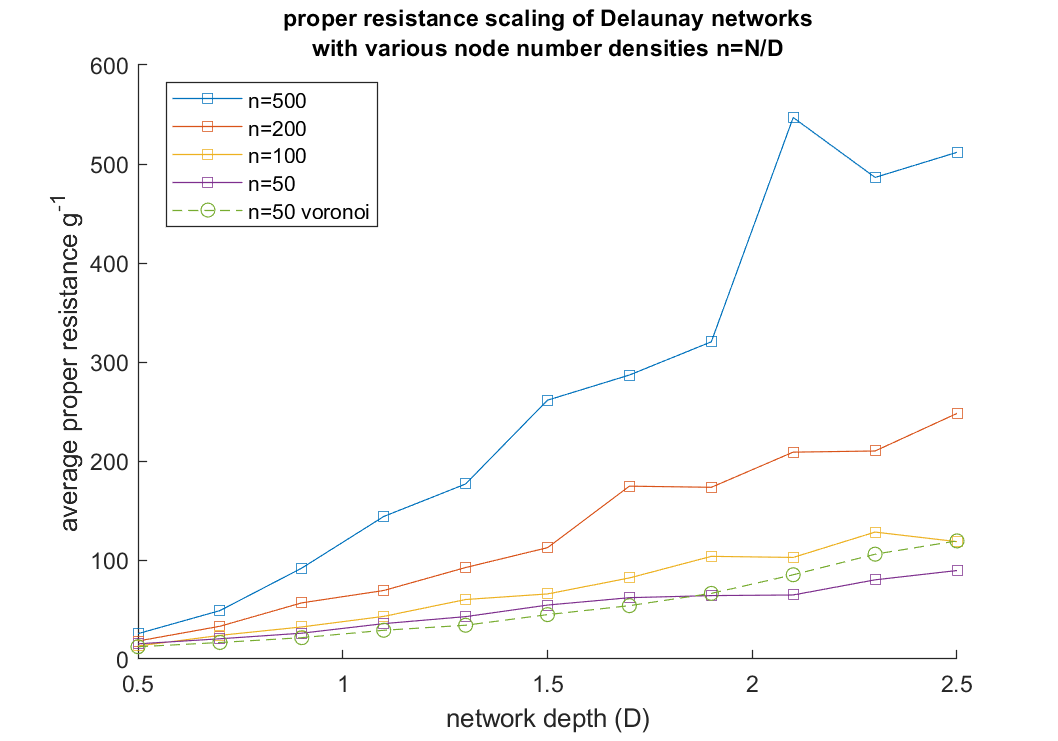
\includegraphics[width=0.8\textwidth]{ch3/fig3/delaunay_scaling.png}
    \caption{$g^{-1}(D)$ for Delaunay networks of various node number densities $n=N/D$, averaged over 1000 realisations of each network. For denser networks, we move away from the linear Ohmic regime into the localised regime. This is computationally expensive so we did not repeat the same analysis for Voronoi graphs, but we have included one (dashed line) to show similar scaling behaviour.} 
    \label{fig:delaunay_scaling}
\end{figure}

Another way to characterise localisation is by fluctuations in the output spectrum \cite{Muller2011}. In contrast to scaling theory, this feature can be observed in a single transport spectrum, without averaging across different realisations of the disordered medium. Fig.\ref{fig:spectrum_microwave} demonstrates this effect observed experimentally in a 3D disordered medium \cite{Genack2005}; Fig.\ref{fig:spectrum_localised} and Fig.\ref{fig:spectrum_diffusive} are results from our simulation.

\begin{figure}[htp]
  \centering
    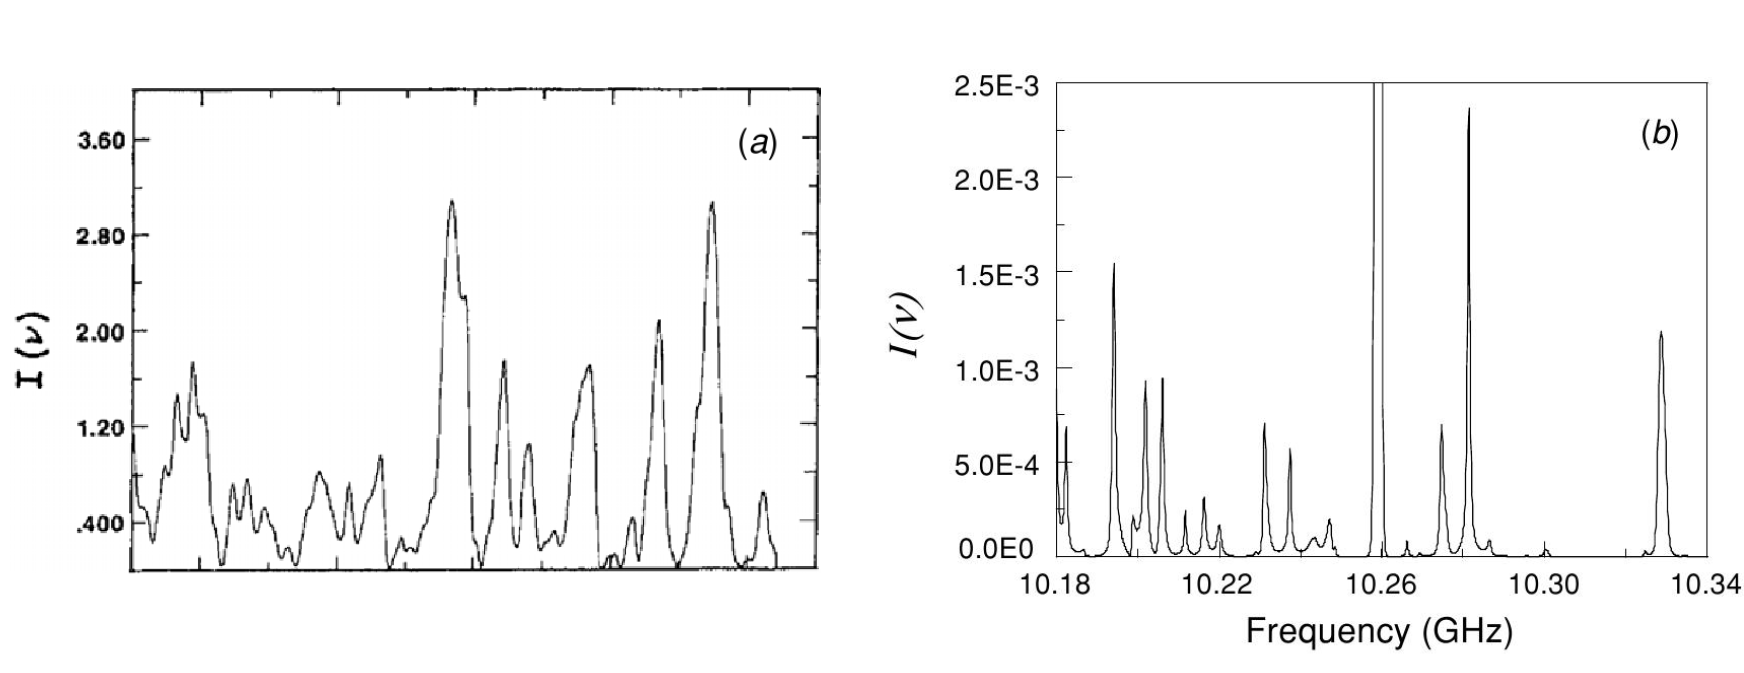
\includegraphics[width=0.9\textwidth]{ch3/fig3/spectrum_microwave.jpg}
    \caption{Transmitted microwave intensity spectra; the disordered medium is aluminium spheres contained in a copper tube. The diffusive regime (a) has broader spectral peaks compared with the sharp fluctuations in the localised regime (b). \cite{Genack2005}} 
    \label{fig:spectrum_microwave}
\end{figure}


\begin{figure}[hbp]
  \centering
    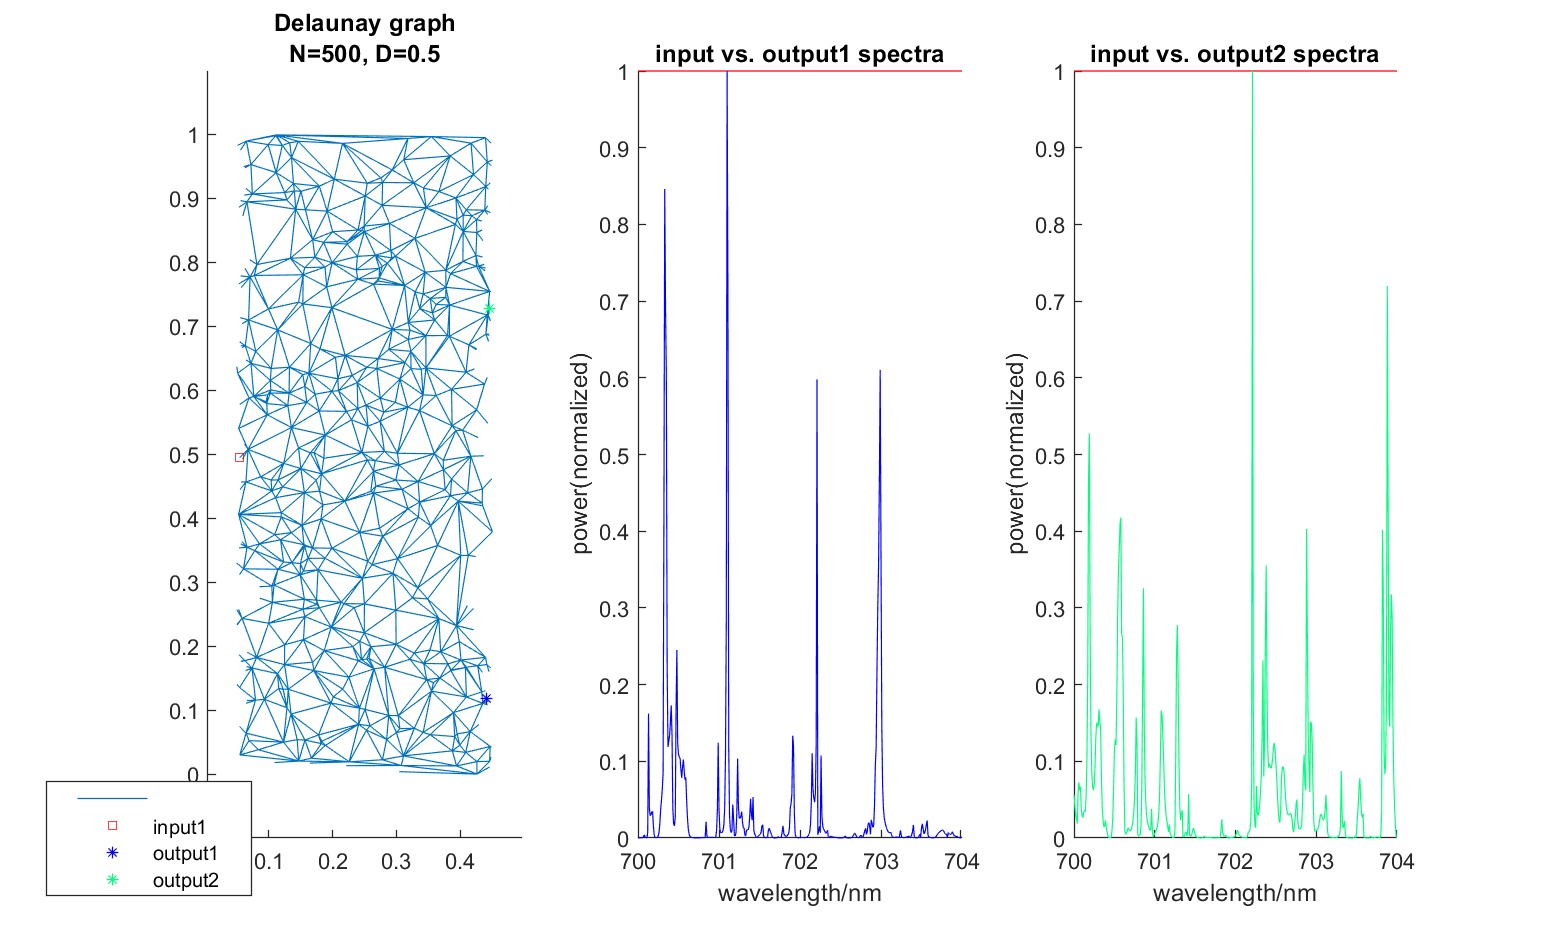
\includegraphics[width=0.95\textwidth]{ch3/fig3/example2_spectra_N500D05d.png}
    \caption{Normalised output spectra at two different output ports on a localised network ($n=1000$). The input is a uniform spectrum across $700\mu m-704\mu m$ injected into the edge labelled with a red marker. The output ports are labelled in dark blue and green.The two outputs have different spectral profiles, but both contain very sharp peaks.} 
    \label{fig:spectrum_localised}
\end{figure}


\begin{figure}[h]
  \centering
    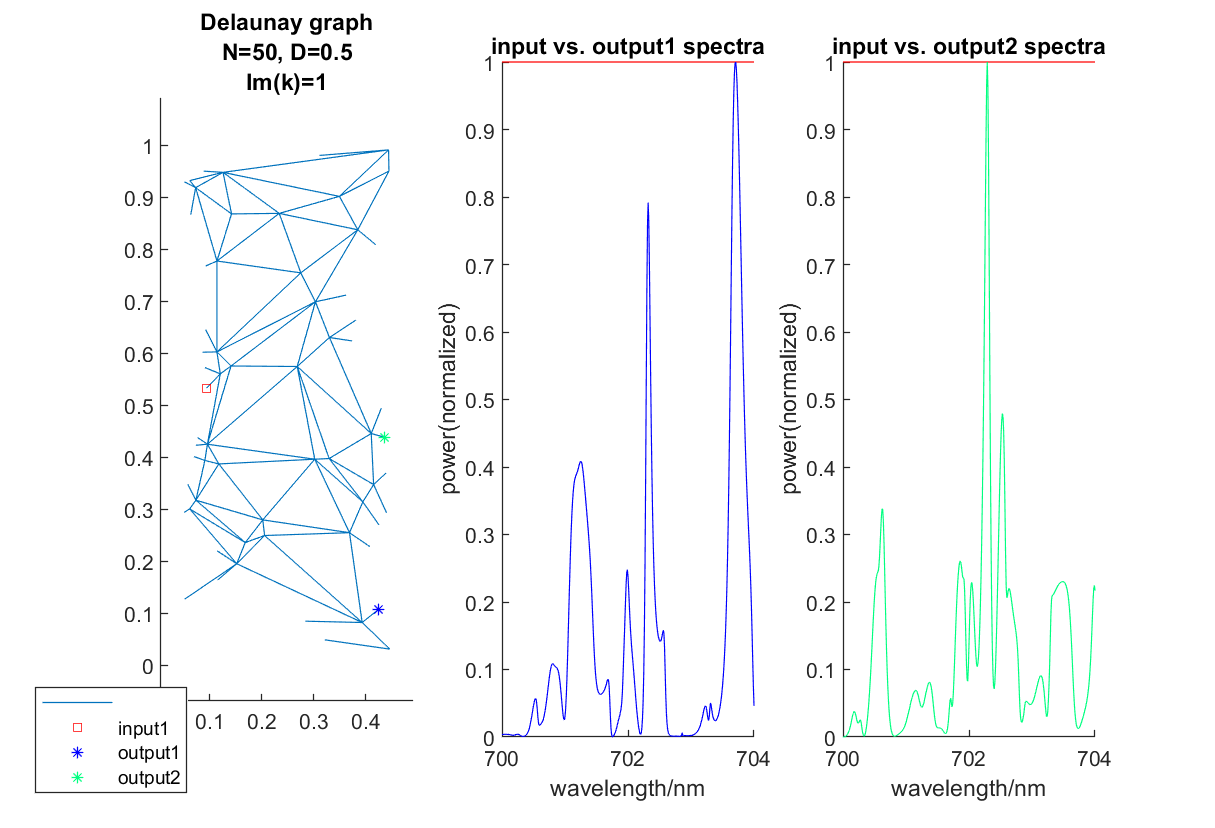
\includegraphics[width=0.95\textwidth]{ch3/fig3/example2_spectra_N50D05d.png}
    \caption{Same analysis as in Fig.\ref{fig:spectrum_localised}, but on a diffusive network ($n=100$). The transmission spectra have significantly broader peaks, similar to that in Fig.\ref{fig:spectrum_microwave}.} 
    \label{fig:spectrum_diffusive}
\end{figure}



\section{Transmission and response modes}
Statistical analysis (e.g.resistance scaling) of complex disordered systems can illustrate their universal properties. However, for the purpose of light state engineering using complex networks, we deal with individual realisations of such networks instead of a large collection of them. We will therefore zoom in again and look at response mode structures within individual networks (cf. section \ref{sec:response_mode_def}).

We will look at two types of network responses, whose intensity profile throughout the entire network (not just the input and output ports) are referred to as \textit{response modes} and \textit{channel modes}. Response modes are columns in the response matrix $R$ defined in Eq.\ref{eq:R}; they are field distributions within a network generated by injecting a unit-intensity input at a single input port. Given $R$ we can obtain the transmission matrix $T$, and singular value decomposition (SVD) yields
\begin{equation}
    \label{eq:T_SVD}
    T = USV^\dagger,
\end{equation}
where $U$, $V$ are unitary and $S$ is diagonal. A channel mode is the network response generated by injecting fields across the input ports given by a column in $V$, i.e. a right eigenvector of $T$. Each channel mode has conductance given by the diagonal elements of $S$. Fig.\ref{fig:response_mode_examples} and Fig.\ref{fig:channel_mode_examples} show examples of both types of modes. To characterise the transport property of each setup, we consider the \textit{transmission}, which is simply the transmitted power, or intensity (elements of $T$ squared). Unless otherwise specified, the term refers to total transmission, i.e. sum of output intensities at all output ports.

\vspace{1cm}
\begin{figure}[h]
    \centering
    \begin{subfigure}[b]{0.4\textwidth}
        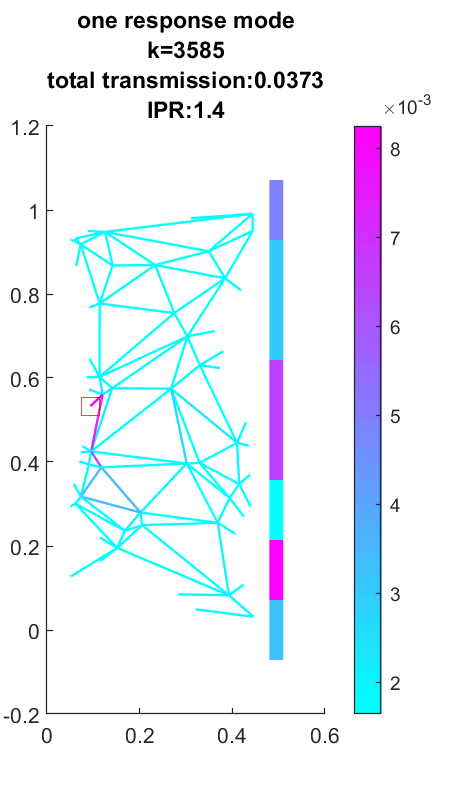
\includegraphics[width=\textwidth]{ch3/fig3/response_mode_N50D05d.png}
        %\caption{}
        %\label{fig:gull}
    \end{subfigure}
~\quad\quad
    \begin{subfigure}[b]{0.4\textwidth}
        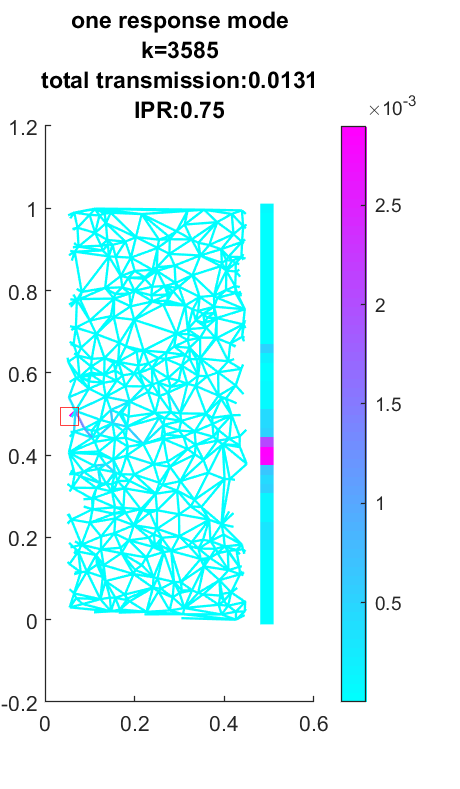
\includegraphics[width=\textwidth]{ch3/fig3/response_mode_N500D05d.png}
        %\caption{}
    \end{subfigure}
    \caption{Example response modes; these are the same networks and input ports as in Fig.\ref{fig:spectrum_localised} and Fig.\ref{fig:spectrum_diffusive}. Colours on each network show relative average field intensities on the edges, and the coloured strip on the right shows spatial distribution of output intensities (location not perfectly aligned with output ports). Colourbar shows scale for the output distribution.}\label{fig:response_mode_examples}
\end{figure}


\begin{figure}[htp]
    \centering
    \begin{subfigure}[b]{0.4\textwidth}
        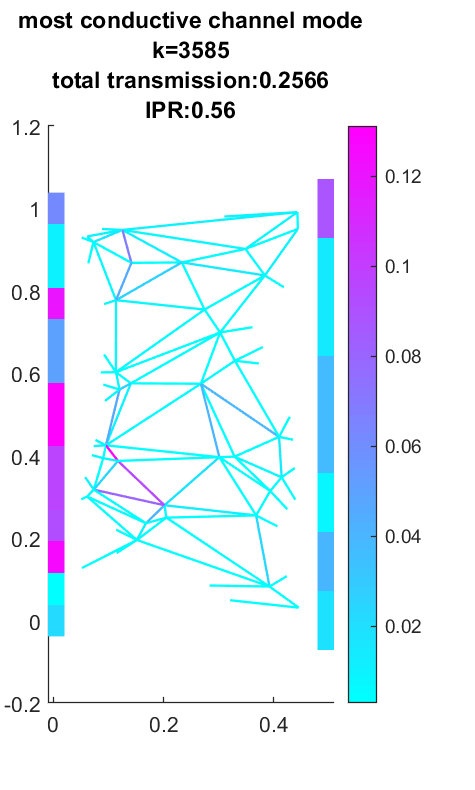
\includegraphics[width=\textwidth]{ch3/fig3/channel_mode_N50D05d.png}
        %\caption{}
        %\label{fig:gull}
    \end{subfigure}
~\quad\quad
    \begin{subfigure}[b]{0.4\textwidth}
        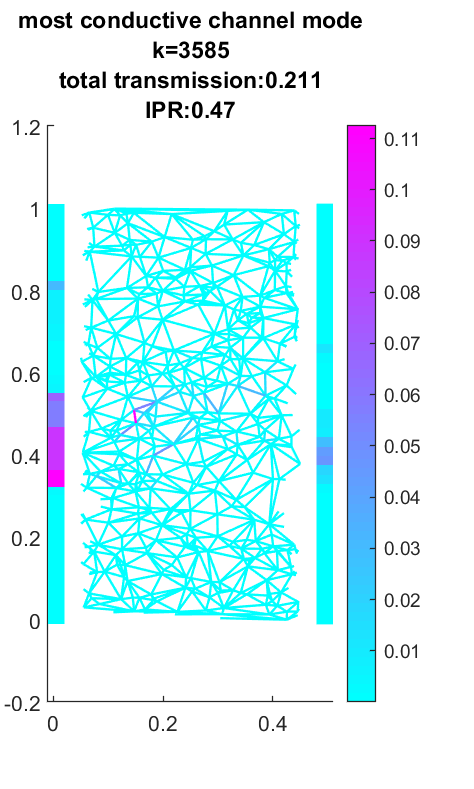
\includegraphics[width=\textwidth]{ch3/fig3/channel_mode_N500D05d.png}
        %\caption{}
    \end{subfigure}
    \caption{Example channel modes. The coloured strip to the left of each network plots the input intensities of a right eigenvector of $T$.}\label{fig:channel_mode_examples}
\end{figure}


\begin{figure}[hbp]
    \centering
    \begin{subfigure}[b]{0.4\textwidth}
        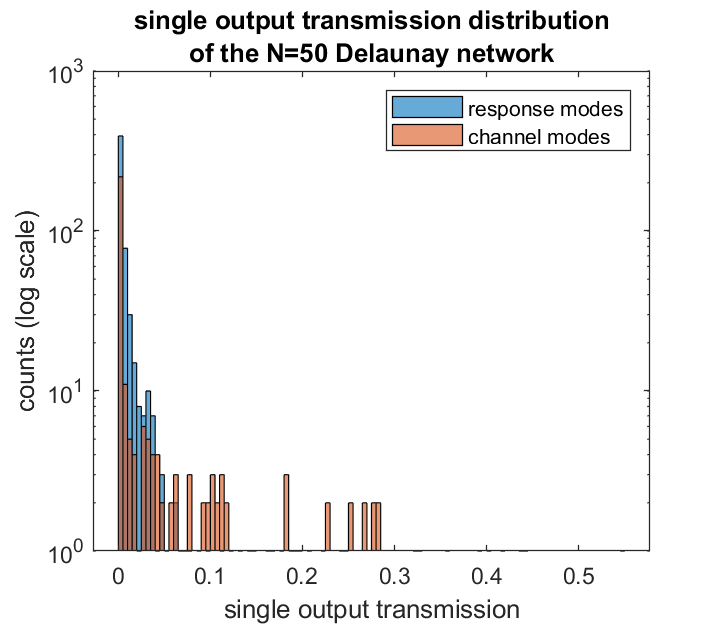
\includegraphics[width=\textwidth]{ch3/fig3/N50d_singleT.png}
        %\caption{}
        %\label{fig:gull}
    \end{subfigure}
~\quad\quad
    \begin{subfigure}[b]{0.4\textwidth}
        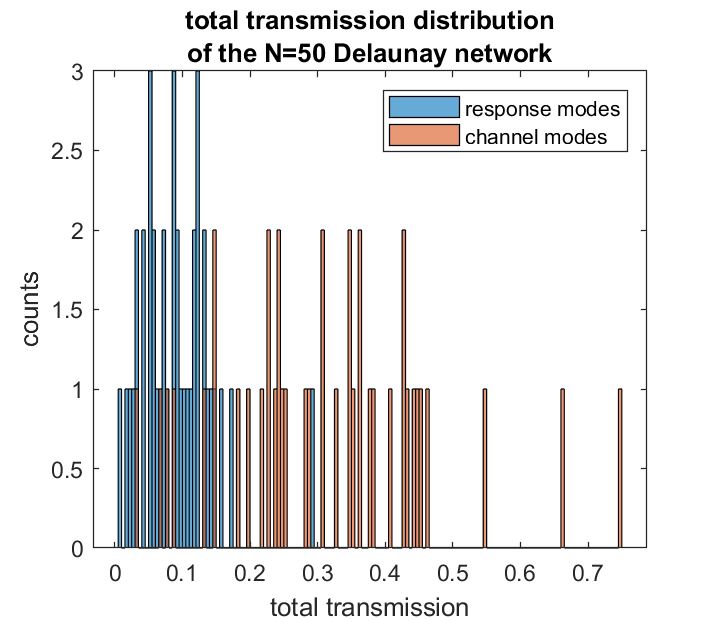
\includegraphics[width=\textwidth]{ch3/fig3/N50d_totalT.png}
        %\caption{}
    \end{subfigure}
    \caption{Transmission distribution across a range of $k$'s for the $N=50$ network from above. Left figure looks at transmitted intensities at individual output ports; right figure looks at the total transmission. Note that the channel modes achiever better transmission by utilising wavefront shaping.}\label{fig:N50_T_hist}
\end{figure}

\begin{figure}[ht]
    \centering
    \begin{subfigure}[b]{0.4\textwidth}
        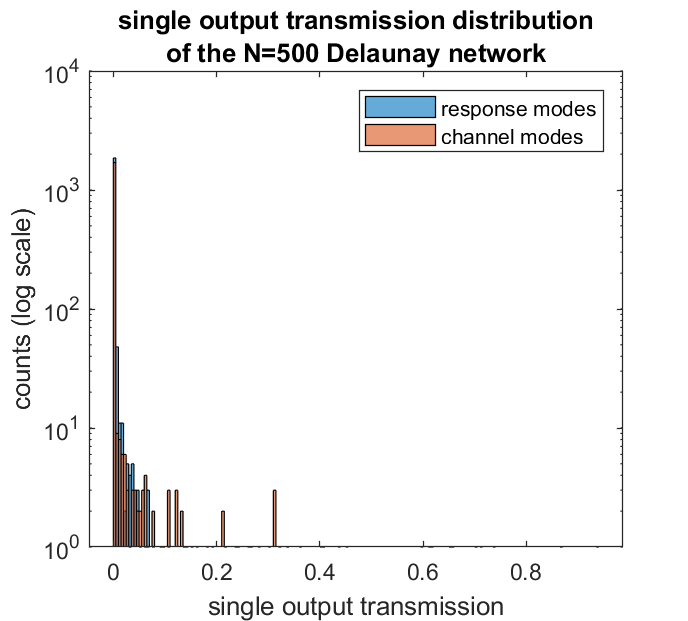
\includegraphics[width=\textwidth]{ch3/fig3/N500d_singleT.png}
        %\caption{}
        %\label{fig:gull}
    \end{subfigure}
~\quad\quad
    \begin{subfigure}[b]{0.4\textwidth}
        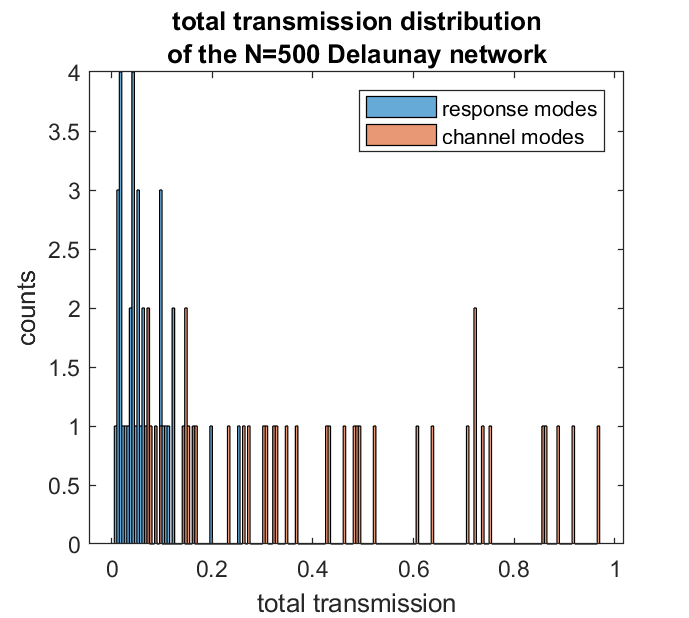
\includegraphics[width=\textwidth]{ch3/fig3/N500d_totalT.png}
        %\caption{}
    \end{subfigure}
    \caption{Transmission distribution across a range of $k$'s for the $N=500$ network from above. Although this is a localised network, channel modes still achieve high overall transmission.}\label{fig:N500_T_hist}
\end{figure}


We look at transmission of the two example networks at a range of $k$'s corresponding to wavelengths $\lambda \in[ 500\mu m , 890 \mu m]$. The resulting transmission distributions are shown in Fig.\ref{fig:N50_T_hist}, Fig.\ref{fig:N500_T_hist}. An important observation is that by picking out the most conductive channel modes using wavefront shaping, one can achieve high transmission even in a localised network.

\subsection{Mode size and transmission}
One feature of interest is to look at the size of a response or channel mode in relation to its transmission. Mode size is characterised by inverse participation ratio (IPR), 
\begin{equation}
    \label{eq:IPR}
    IPR = \frac{\int (E^2)^2 dx}{(\int E^2 dx)^2},
\end{equation}
Where the integral is over $E$ field on an entire network. This is the integral over density of $E^2$, analogous to the definition of purity of a density operator in quantum information. IPR captures the degree of localisation of a field distribution (mode): the higher the IPR, the more spatially confined a mode is. Fig.\ref{fig:spectrum_localised} and Fig.\ref{fig:spectrum_diffusive} show the corresponding IPR for each example.

\begin{figure}[htp]
  \centering
    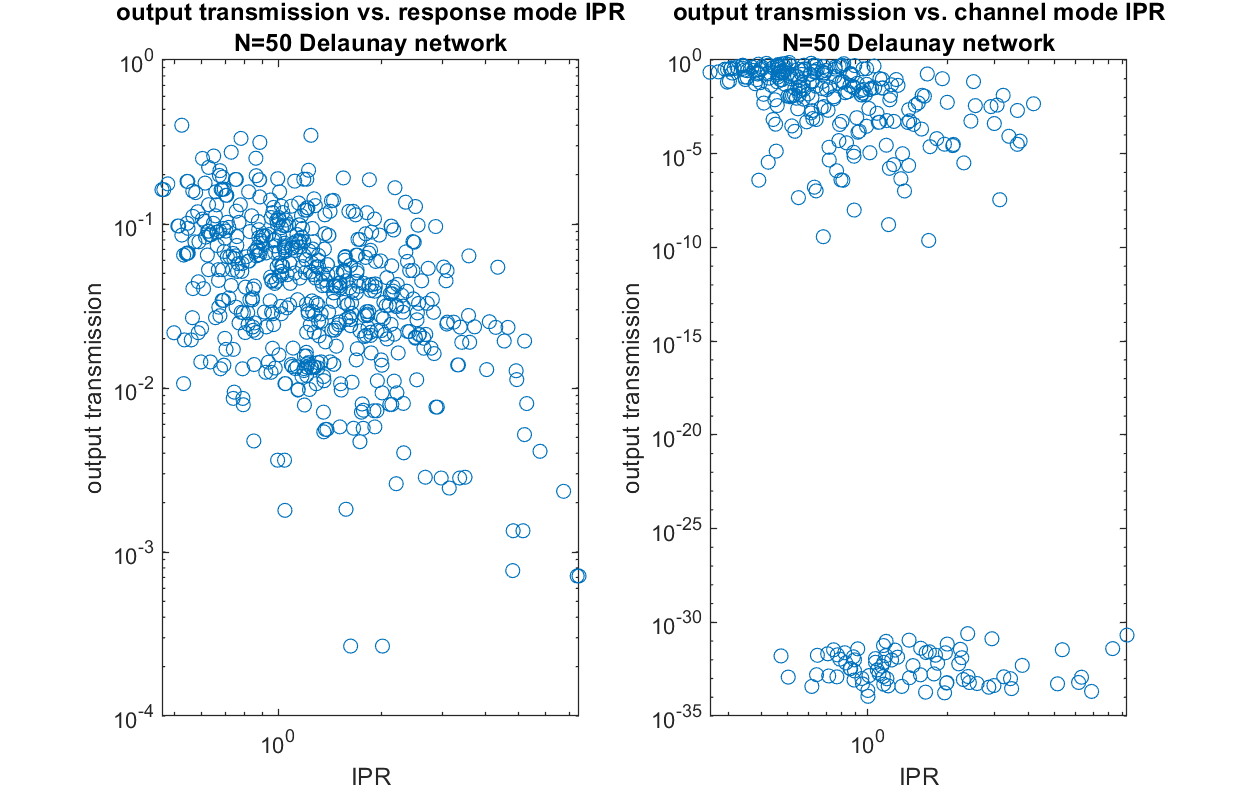
\includegraphics[width=0.8\textwidth]{ch3/fig3/IPRvsT_N50dexample.png}
    \caption{Output transmissions vs. IPR for the $N=50$ network from above. We see the intuitive correlation that the higher the IPR, i.e. the more localised the modes are, the less they transmit. Note that the distribution along the $y$-axis is the same as that shown in Fig.\ref{fig:N50_T_hist}. As seen before, the channel modes result in concentrated output intensity in some output ports (with overall higher transmission) and zero in others.} 
    \label{fig:IPRvsT_N50}
\end{figure}

\begin{figure}[hbp]
  \centering
    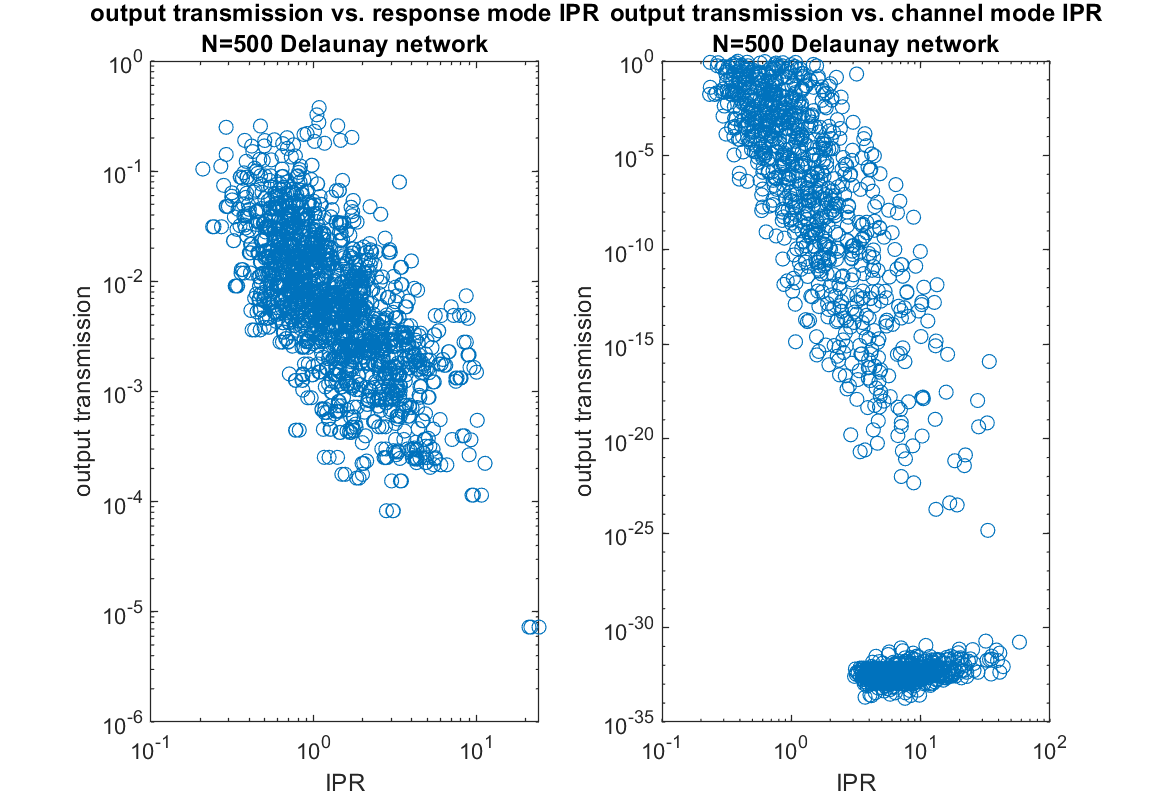
\includegraphics[width=0.8\textwidth]{ch3/fig3/IPRvsT_N500dexample.png}
    \caption{Same analysis as above but for the $N=500$ network. In the localised regime we see a stronger correlation between transmission and IPR.} 
    \label{fig:IPRvsT_N500}
\end{figure}

\begin{figure}[htp]
  \centering
    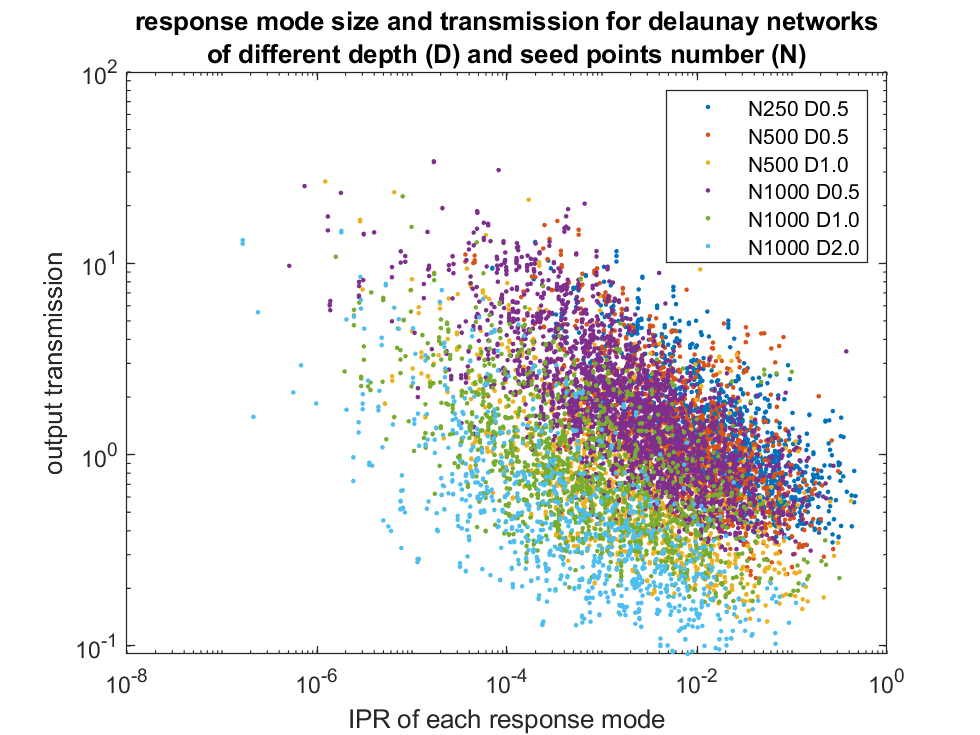
\includegraphics[width=0.75\textwidth]{ch3/fig3/compare_delaunay.png}
    \caption{The same output transmission vs. IPR analysis as above, but for a range of Delaunay graphs with different $N$ and $D$ values. Note that in terms of output transmission, scaling up networks with the same density $n=N/D$ (shown here in dark blue, yellow, and light blue) has a stronger effect than stretching networks of the same $N$ to different sizes (purple, green, and light blue). Networks of the same $D$ but different $n$ (dark blue, red, purple) show greater variation in IPR than transmission. We also observe as before a stronger correlation between transmission and IPR for networks with larger $n$.} 
    \label{fig:compare_delaunay}
\end{figure}

\begin{figure}[hbp]
  \centering
    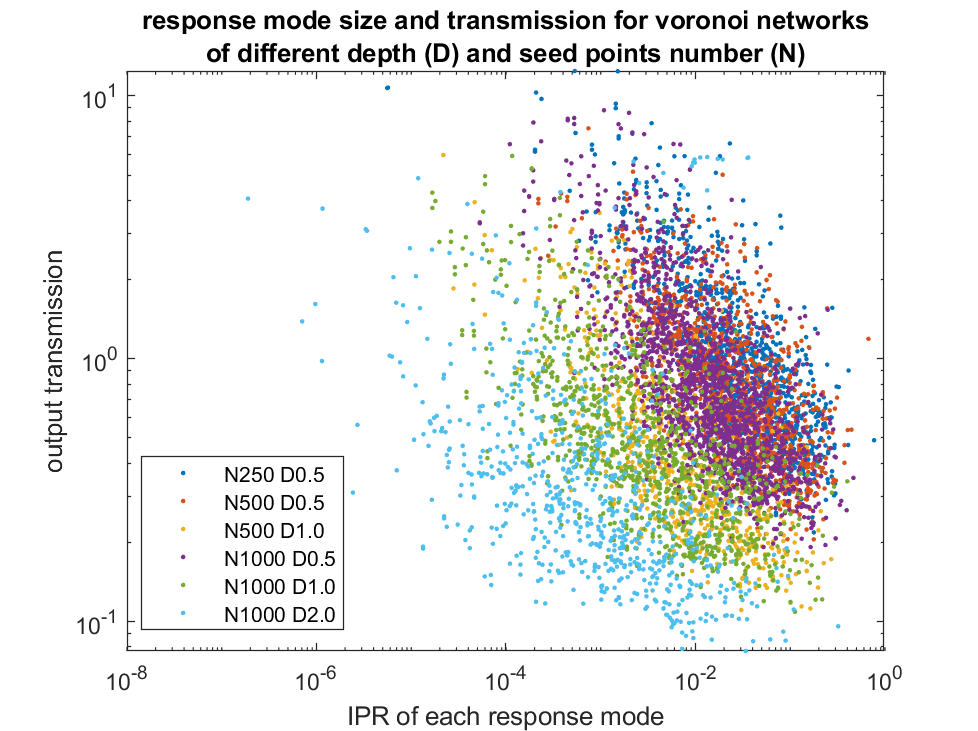
\includegraphics[width=0.75\textwidth]{ch3/fig3/compare_voronoi.png}
    \caption{Same as Fig.\ref{fig:compare_delaunay} but for Voronoi networks. A similar trend is observed.} 
    \label{fig:compare_voronoi}
\end{figure}

In particular, we look at the correspondence between the IPR of a response or channel mode in relation to a) its transmission in individual output ports, and b) the total transmission. We observe in all cases that a more localised mode (with higher IPR) generally has lower transmission than a less localised one (Fig.\ref{fig:IPRvsT_N50} and Fig.\ref{fig:IPRvsT_N500}), and the effect is stronger in a larger network. This makes sense since for a network in the localised regime, a spatially confined (localised) mode is harder to access simultaneously by the inputs on the left and the outputs on the right.
Fig.\ref{fig:compare_delaunay} and Fig.\ref{fig:compare_voronoi} conduct the same analysis on a range of Delaunay and Voronoi networks with varying $N$, $D$, and $n=N/D$. For both types of networks we find that varying $D$ while keeping $n$ constant has the greatest effect on transmission, while varying $n$ for the same $D$ has a larger effect on IPR than transmission. This can be understood by noting that $n$ sets the degree of disorder, and thus $\xi_{loc}$, and that transmission is determined by the ratio $D/\xi_{loc}$ (cf. Eq.\ref{eq:scaling}).

\subsection{$k$-dependence}
As we have seen (e.g. Fig.\ref{fig:spectrum_localised}) the networks, particularly those in the localised regime, display highly $k$-dependent transport behaviour. We look at the channel mode profiles at various $k$ in various networks in figures \ref{fig:kmodes_N50D05d}, \ref{fig:kmodes_N500D05d}, \ref{fig:kmodes_N500D05v}, and \ref{fig:kmodes_N1000D20V}.

These examples show a wide range of channel mode behaviours, and demonstrate the different frequency response in different networks. More interestingly, we see the open channels couple to resonant, localised network modes. A feature of note is that for channels with localised field intensity within the network and high transmission (e.g. $k=3642$ in Fig.\ref{fig:kmodes_N500D05v} and Fig.\ref{fig:kmodes_N1000D10V}), the localised network modes tend to be in the middle of the network along the $x$-axis. This is because a mode in the middle is more likely to be simultaneously accessed by open ports on both left and right. In the context of electrons in solids (i.e. wavefunctions instead of electromagnetic waves), this means it is easier to achieve transmission by tunnelling into and out of a mode localised in the middle \cite{Muller2011}.

\begin{figure}[htp]
  \centering
    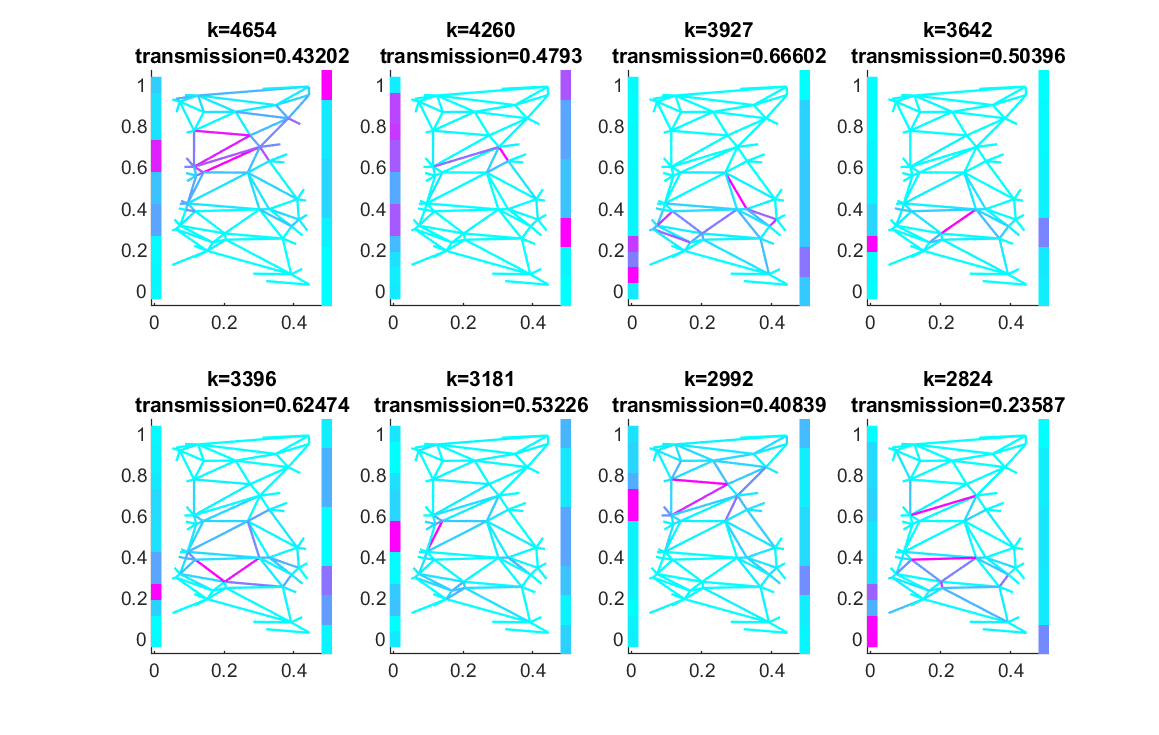
\includegraphics[width=0.8\textwidth]{ch3/fig3/kmodes_N50D05d.png}
    \caption{Input, output, and mode profiles for the most conductive channel mode at various $k$'s, for the same $N=50, D=0.5$ Delaunay network as before. This is a diffusive network; we see no spatial confinement of channel modes and relatively high transmission in all cases.} 
    \label{fig:kmodes_N50D05d}
\end{figure}

\begin{figure}[hbp]
  \centering
    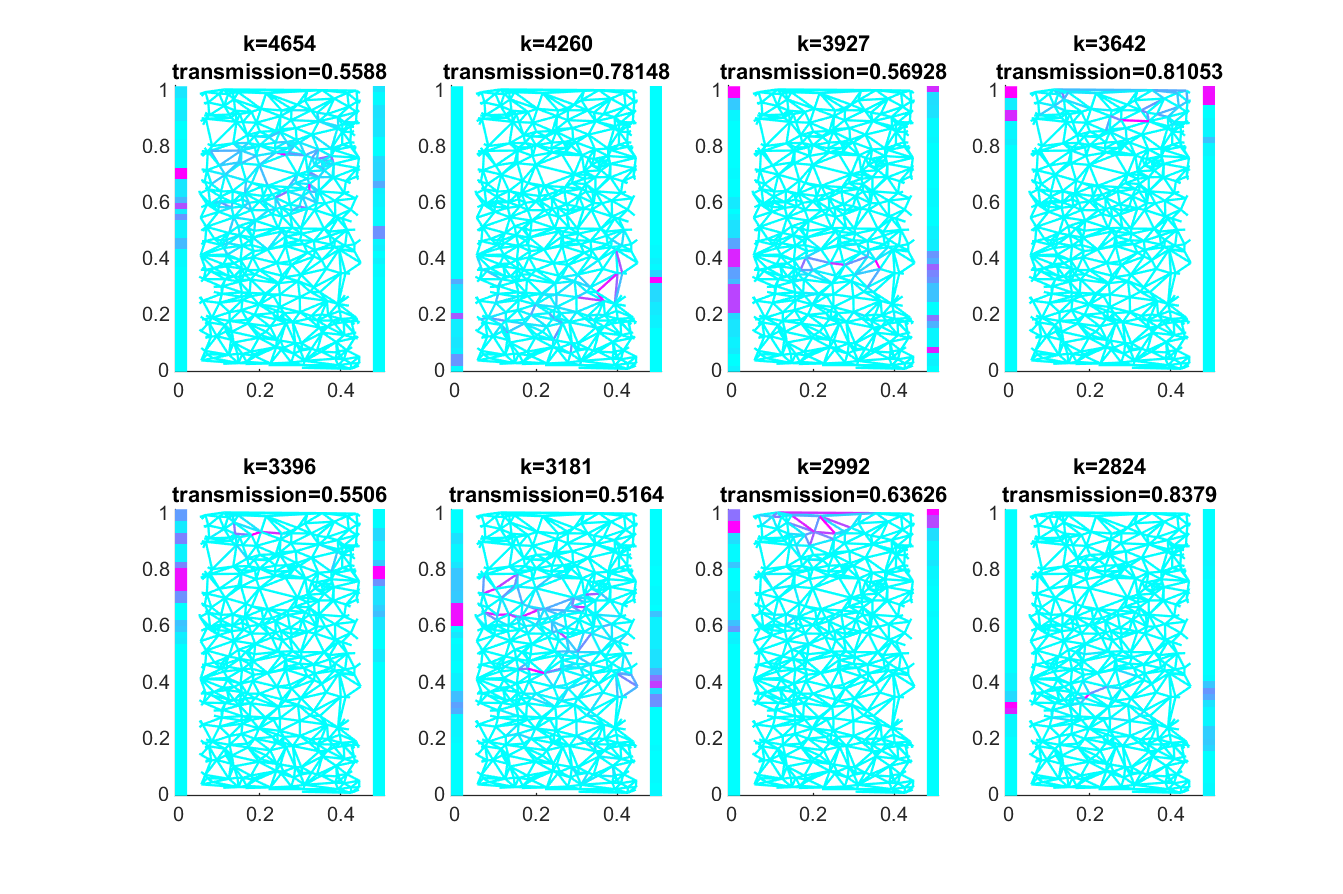
\includegraphics[width=0.9\textwidth]{ch3/fig3/kmodes_N500D05d.png}
    \caption{Input, output, and mode profiles for the most conductive channel mode at various $k$'s, for the same $N=500, D=0.5$ Delaunay network as before. We begin to see localisation effects. For the $k=2824$ example, field intensity is concentrated in a small region in the network, but the total transmission is very high: both the input and output ports are coupled to a network mode in the middle.} 
    \label{fig:kmodes_N500D05d}
\end{figure}

\begin{figure}[htp]
  \centering
    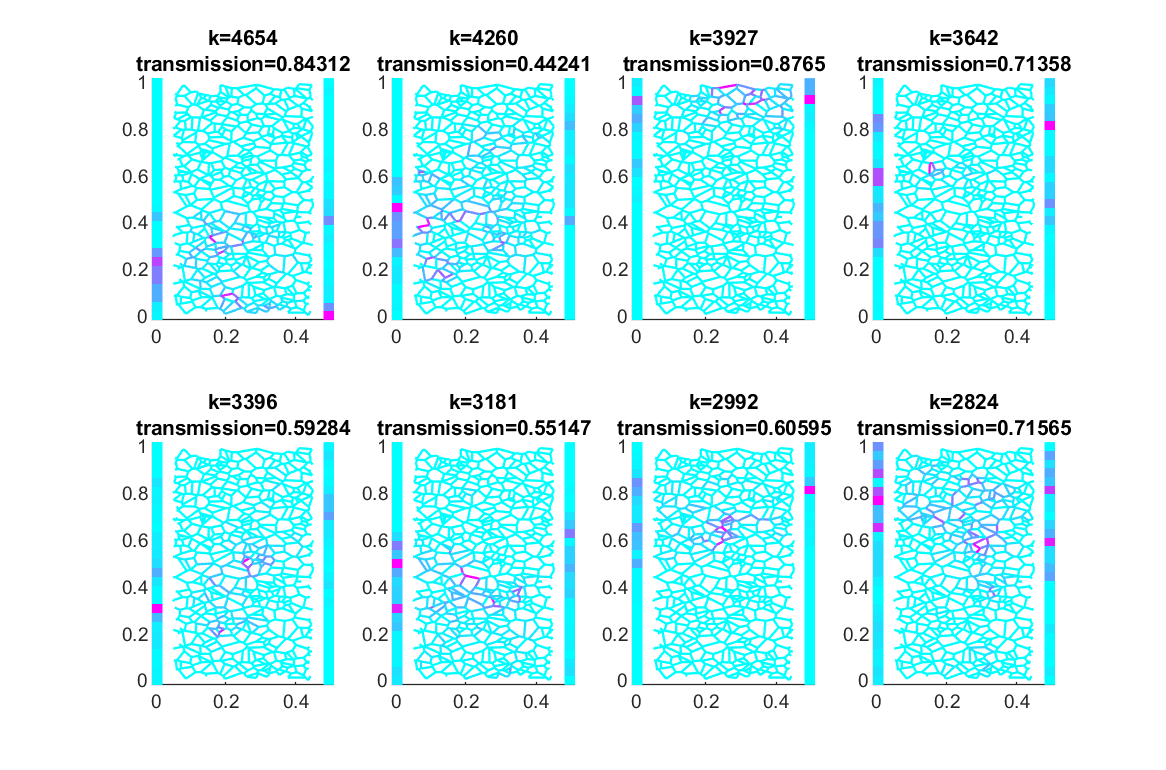
\includegraphics[width=0.9\textwidth]{ch3/fig3/kmodes_N500D05v.png}
    \caption{Same as above but for the $N=500, D=0.5$ Voronoi network. In the $k=3642$ example, a wide range of input ports is used to couple to a localised mode and achieve high transmission.} 
    \label{fig:kmodes_N500D05v}
\end{figure}

\begin{figure}[hbp]
  \centering
    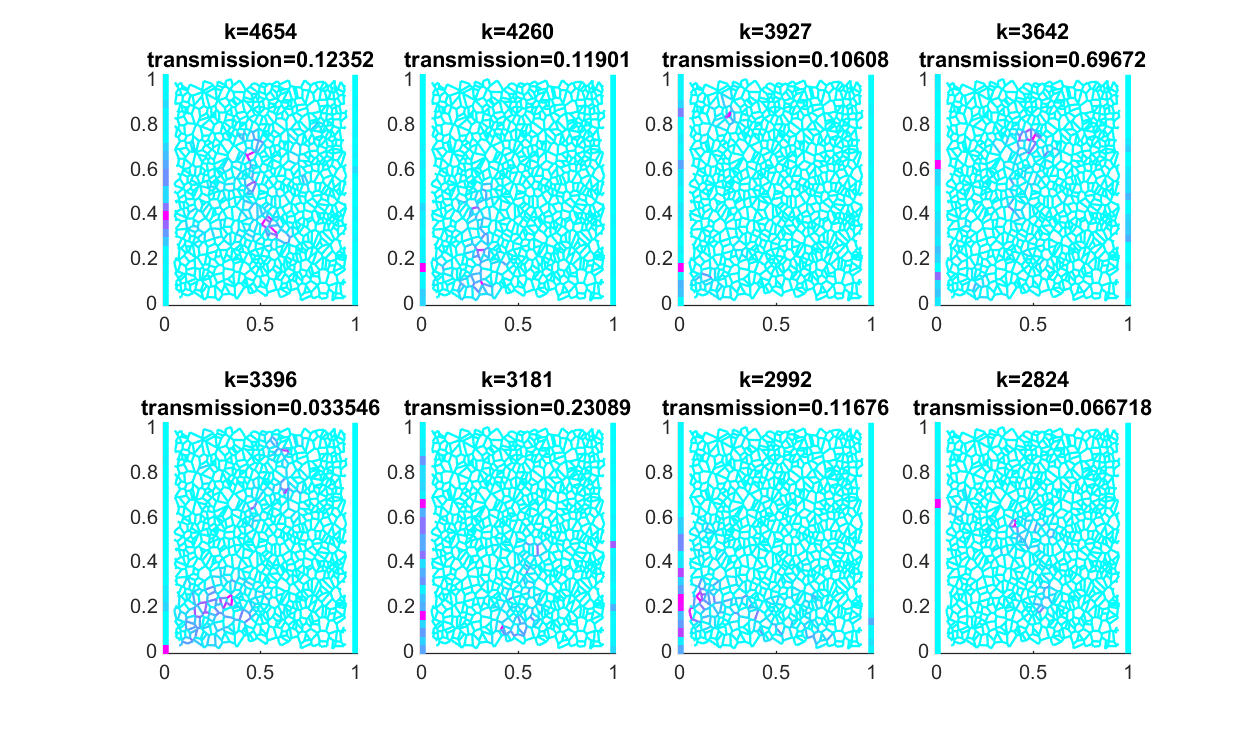
\includegraphics[width=1\textwidth]{ch3/fig3/kmodes_N1000D10v.png}
    \caption{$N=1000, D=1.0$ Voronoi network. The more conductive channels tend to couple to network modes in the middle (e.g. $k=2642$).} 
    \label{fig:kmodes_N1000D10V}
\end{figure}



\section{Absorption and Loss}
Experimental realisations of complex nanophotonic networks will inevitably have imperfections. One likely imperfection is loss, either by absorption of the material or out-of-plane scattering. Absorptions in waveguide materials such as silicon nitride are low, but large out-of-plane scattering at nodes have been observed in similar random networks \cite{Gaio2017}. Loss is an important effect to study because the theory of coherent multiple scattering holds for \textit{elastic} scattering, therefore localisation theory only holds for sufficiently low losses \cite{Muller2011}.

Loss is introduced into our model in two ways. The simplest approach is to add a positive imaginary part to the wavenumber $k$. This most directly models uniform absorption along the edges, but can also serve as an approximation that distributes any loss uniformly across the network. The second approach introduces loss at each node by modifying the second continuity condition Eq.\ref{eq:in=out}:

\begin{equation}
    \label{eq:in=out+loss}
    [1-\textrm{loss}(x_i)] \cdot \sum \Psi_{\textrm{ingoing}} (x_i) = \sum \Psi_{\textrm{outgoing}} (x_i).
\end{equation}

This is a more realistic model which allows us to introduce different losses at each node. Fig.\ref{fig:edge_loss} and Fig.\ref{fig:node_loss} show that localisation effects are smeared out for sufficiently large losses using either approach (cf. Fig.\ref{fig:spectrum_microwave}).

Broadened spectral peaks for transmission though a lossy network can also be understood using the physical pictures introduced in section \ref{sec:physical_picture}. In particular, we can view the modes of a network as resonant modes supported by a collection of coupled ring resonators. If these resonators are lossy, the low Q factors will show up as broadened peaks in a transmission spectrum.

\begin{figure}[htp]
  \centering
    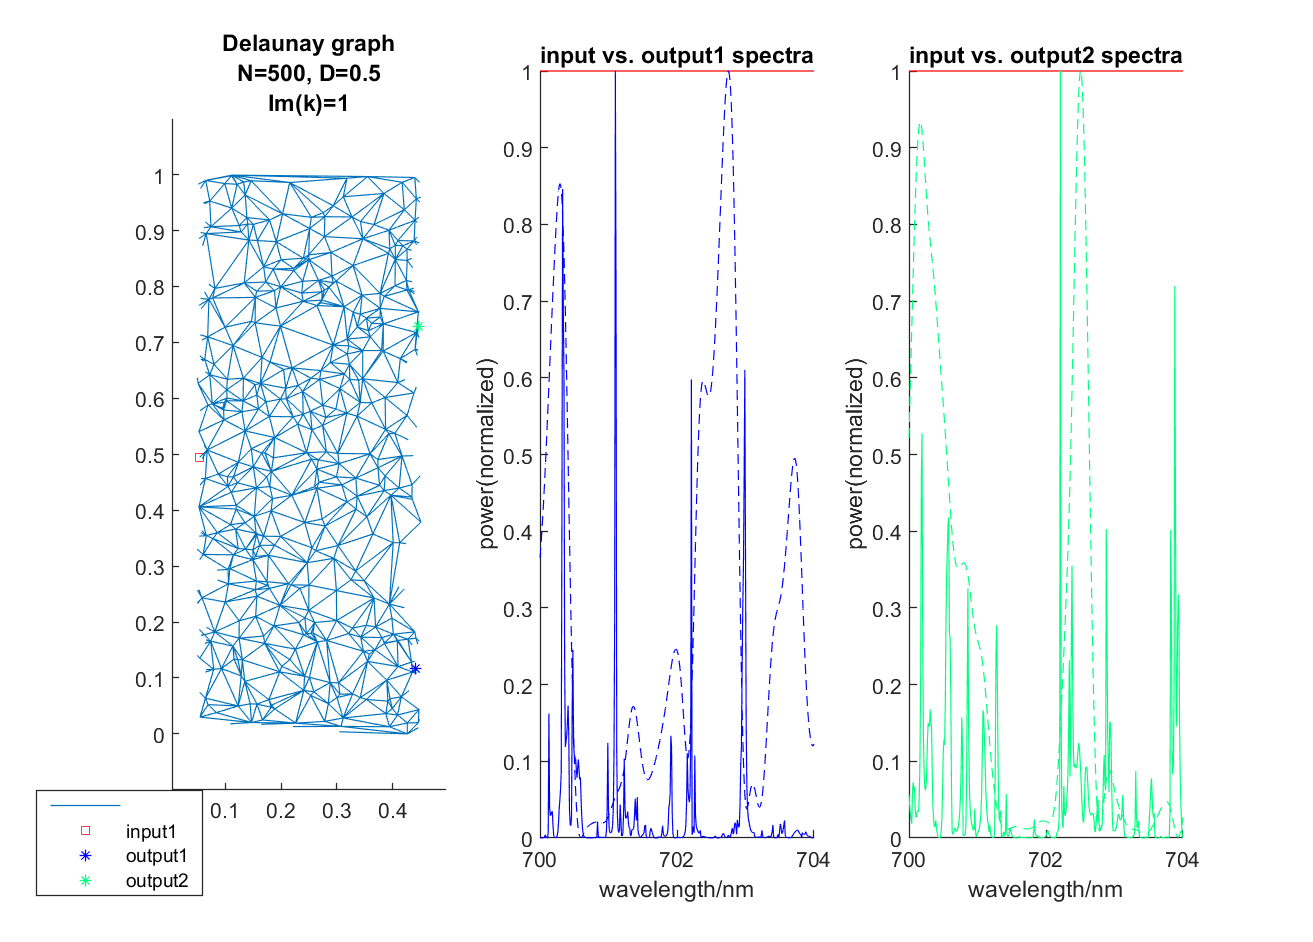
\includegraphics[width=0.8\textwidth]{ch3/fig3/edge_loss.png}
    \caption{Effect of loss on transmission spectra by adding an imaginary part to $k$. Broadening of the peaks (this is the same example as in Fig.\ref{fig:spectrum_localised}) signify the absence of localisation. Solid lines show original spectra, dashed lines are modified spectra with loss.} 
    \label{fig:edge_loss}
\end{figure}

\begin{figure}[hbp]
  \centering
    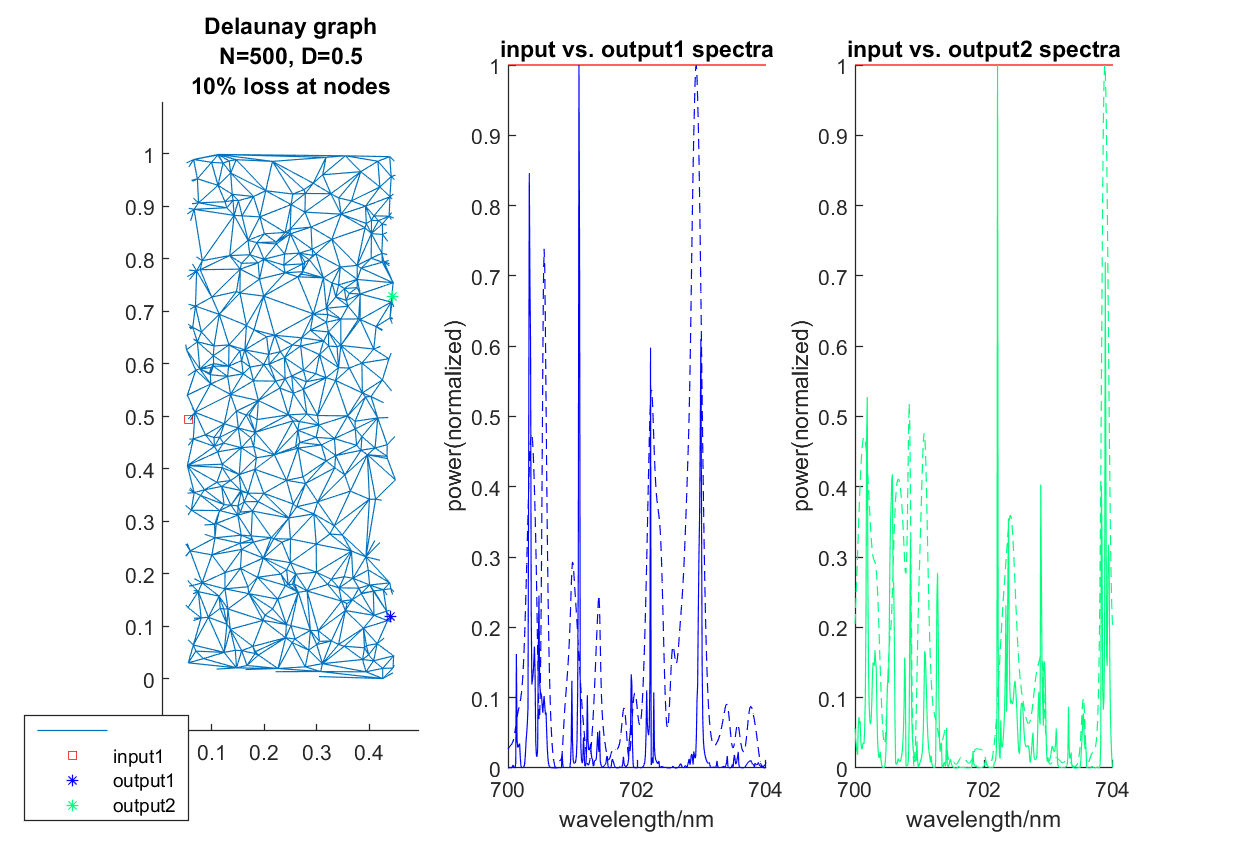
\includegraphics[width=0.8\textwidth]{ch3/fig3/node_loss.png}
    \caption{Loss introduced by adding a $10\%$ loss at each internal node. This shows different modifications to the spectra than the approach in Fig.\ref{fig:edge_loss}, but broadens the spectral peaks nonetheless. Solid lines are oiginal spectra, dashed lines spectra with loss.} 
    \label{fig:node_loss}
\end{figure}


\section{Boson sampling and quantum interference}
We will now introduce quantum interference effects using the approach discussed in section \ref{sec:quantisation}. Namely, we use the same $T$ matrices obtained classically, but treat the output vectors as superpositions of different output locations, and let them interfere as Bosonic field operators.

Interference between two single-photon inputs is investigated as a basic example for quantum phenomena. For the sake of comparison, we use the same $N=50, D=0.5$ Delaunay network as before. The rest of this section looks at three different input configurations.

\begin{itemize}
    \item \textbf{same $k$, same $x$}
    
    The scenario of two indistinguishable photons, i.e. two with the same frequency as well as input location, is a analogous to the Hong-Ou-Mandel effect on a beam-splitter. We have neglected photon/light polarisation so far as it is not modified by the networks. Since the networks are linear, any coherence in polarisation will also be preserved. We will thus assume all photons have the same polarisation and suppress this degree of freedom in the following discussions.
    
    Indistinguishable inputs result in identical output wavefunctions that self-interfere. Given two identical inputs $a^\dagger(x_l,k)$,
    \begin{align}
\label{eq:samexsamek}
        \Phi_{out} &= \bigg(\sum_m c_{lm}a^\dagger(x_m, k)\bigg)^2\\ \nonumber
          &= \sum_m c_{lm}^2 a^\dagger_m a^\dagger_m + 2\sum_{m,n} c_{lm}c_{ln} a^\dagger_m a^\dagger_n
\end{align}
    Where $m,n$ are indices ranging over the input ports, $c_{lm} = T(k)_{m,l}$. In the second line we have abbreviated $a^\dagger(x_m, k) = a^\dagger_m$ since $k$ is unaffected. We have grouped the off-diagonal interference terms together since $a^\dagger_m$ and $a^\dagger_n$ commute for outputs $m \neq n$. Fig.\ref{fig:samexsamek} compares quantum and classical transport.
    
    \begin{figure}[ht]
    \centering
    \begin{subfigure}[b]{0.5\textwidth}
        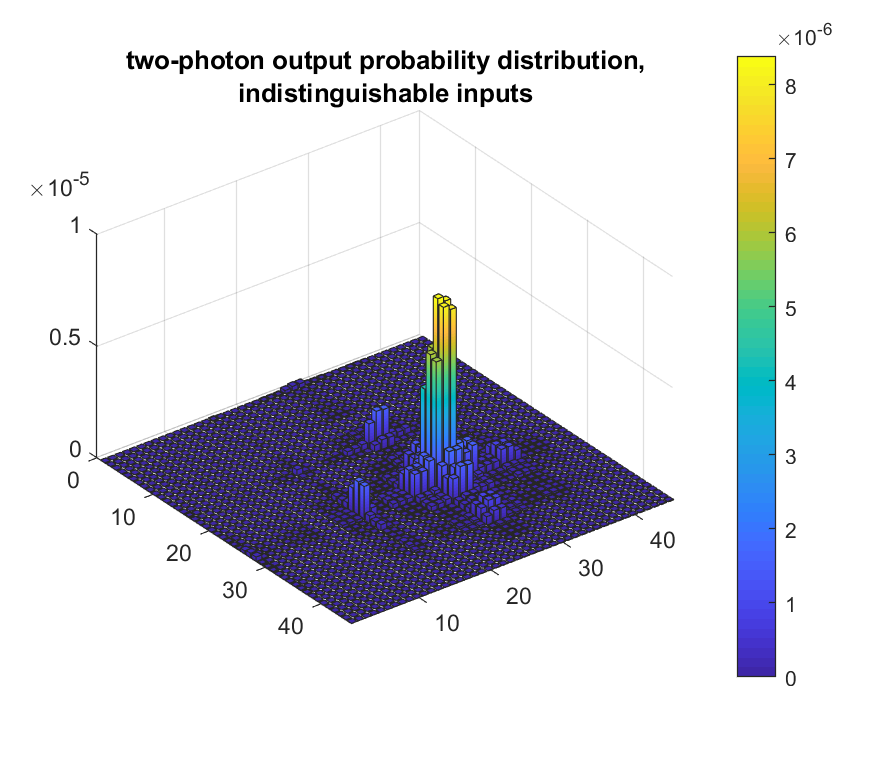
\includegraphics[width=\textwidth]{ch3/fig3/T3585_Q.png}
        %\caption{}
        %\label{fig:gull}
    \end{subfigure}
    ~
    \begin{subfigure}[b]{0.45\textwidth}
        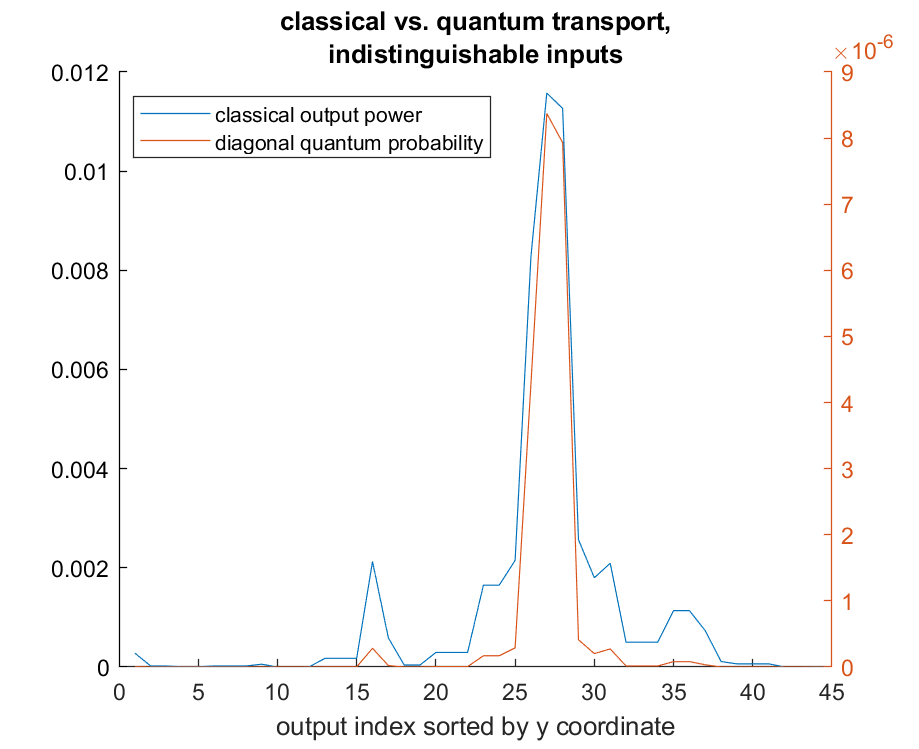
\includegraphics[width=\textwidth]{ch3/fig3/T3585_QvC.png}
        %\caption{}
    \end{subfigure}
    \caption{Quantum interference of two indistinguishable photon inputs, same network and input port as in Fig.\ref{fig:spectrum_localised}, $k=3585$. Left figure shows the quantum output probability distribution, it is symmetrical as expected. Right figure compares the diagonal elements to the classical transport output; there is no pronounced effect like the HOM dip but we do see suppression of certain peaks.}
    \label{fig:samexsamek}
\end{figure}
    
    
    \item \textbf{same $k$, different $x$}
    
    We now consider interference between two photons of the same $k$ injected at different input ports. This is a minimal example of boson sampling using complex networks. Boson sampling is a passive, linear photonic process that is classically hard to simulate, first proposed by S.Aaronson \cite{Aaronson2010}. We inject $p$ photons of the same frequency into a linear optical circuit and observe $p$ photon outputs; this has high computational complexity since bosonic wave equations are symmetric under exchange and computing output probabilities involves computing matrix permanents, a $P\#$ problem \cite{Gard2014}. Example shown in Fig.\ref{fig:diffxsamek}.
    
    \begin{figure}[ht]
    \centering
    \begin{subfigure}[b]{0.5\textwidth}
        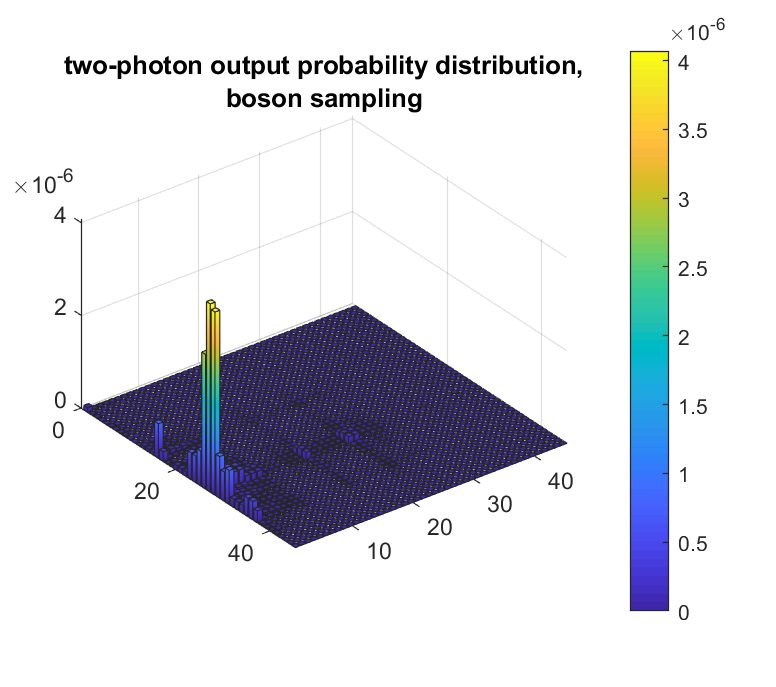
\includegraphics[width=\textwidth]{ch3/fig3/BS_Q.png}
        %\caption{}
        %\label{fig:gull}
    \end{subfigure}
    ~
    \begin{subfigure}[b]{0.4\textwidth}
        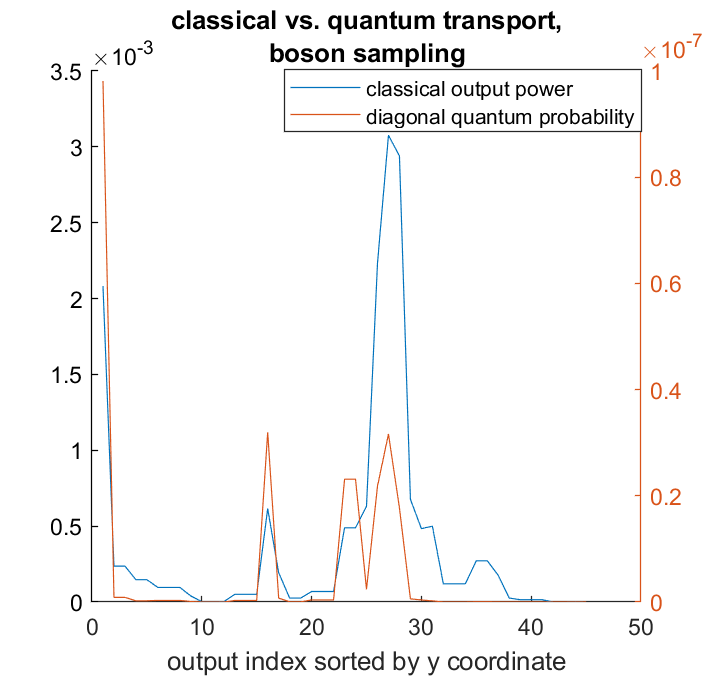
\includegraphics[width=\textwidth]{ch3/fig3/BS_QvC.png}
        %\caption{}
    \end{subfigure}
    \caption{Boson sampling using the same network as above, $k=3585$. The behaviour deviates significantly from classical result.}
    \label{fig:diffxsamek}
\end{figure}
    
    \item \textbf{different $k$, different $x$}
    
    This case is very similar to the same-$k$ boson sampling scenario above. The resulting output probability distributions (referred to as the $P$ matrix) would look the same, except now we would be able to experimentally distinguish events given by $P{i,j}$ and $P_{j,i}$, since they will occupy the same output ports but have different output $k$ orders.

    
    
\end{itemize}